\documentclass[10pt,a4paper]{amsart}
% \usepackage{geometry}\geometry{margin=1.5in}
\usepackage{latexsym, bbm, enumerate, amssymb, amsmath, graphicx, amsthm}
\usepackage{tikz}
% \usepackage[nolists]{endfloat}

\newtheorem{theorem}{Theorem}[section]
\newtheorem{corollary}{Corollary}[theorem]
\newtheorem{lemma}[theorem]{Lemma}
\newtheorem*{remark}{Remark}

% \newcommand{\EE}{{\mathbb{E}}}
\newcommand{\EE}{E}
% \newcommand{\PP}{{\mathbb{P}}}
\newcommand{\PP}{P}
% \newcommand{\E1}{\EE(Y\mid A=1,X)}
% \newcommand{\H}[1]{H^{(1)}_{#1}}
\newcommand{\E}[1]{\EE(Y\mid A=#1,X)}

\DeclareMathOperator{\Var}{Var}
\DeclareMathOperator{\Cov}{Cov}
\DeclareMathOperator{\logit}{logit}
% \renewcommand{\includegraphics}[2][]{\fbox{}}

\begin{document}
\noindent\textbf{Setup.} We have proposed estimating
\[
  p\E0 + (1-p)\E1
  \]
  by
  \[
    \EE(\tilde{Y}\mid X)
  \]
  where
  \[
    \tilde{Y} = \left(\frac{p}{1-p}\right)^{1-2A}Y.
    \]
In approach \#1 (Tsiatis's approach), analysts compute $\E0$ on the
control data $\{(Y_i,X_i): A_i=0\}$, obtaining some regression
function $\hat{f}_0(X)$, and analogously for the case data to get
$\hat{f}_1(X)$. The estimates
\[
  p\hat{f}_0(X_i) + (1-p)\hat{f}_1(X_i)
\]
are used in an estimating equation our actual target, the ATE. In
approach \#2, our
approach, the analysts uses the transformed data
$\{(\tilde{Y}_i,X_i)\}$ to estimate some $\hat{f}(X)$, which is then
used in the estimating equation.\\

\noindent\textbf{Simulation.} Suppose the data follows a simple linear
model with no interactions,
\[
  Y = \alpha A + \beta^T X + \epsilon
\]
with $(A,X,\epsilon)$ mutually independent. Then the true value of
$p\E0 + (1-p)\E1$ is $p(\beta^TX)+(1-p)(\alpha+\beta^TX)$ . I compare the efficiency of the two
approaches by comparing the MSEs of the two estimators. (These MSEs are
directly related to the finite-sample variance of the true target the ATE.) It seems that
our approach (the ``simple'' estimator) is less efficient than the
two-regression approach (the ``combined'' estimator) for $p\neq 1/2$
(figs \ref{fig:1},\ref{fig:2}).
\begin{figure}[h!]
  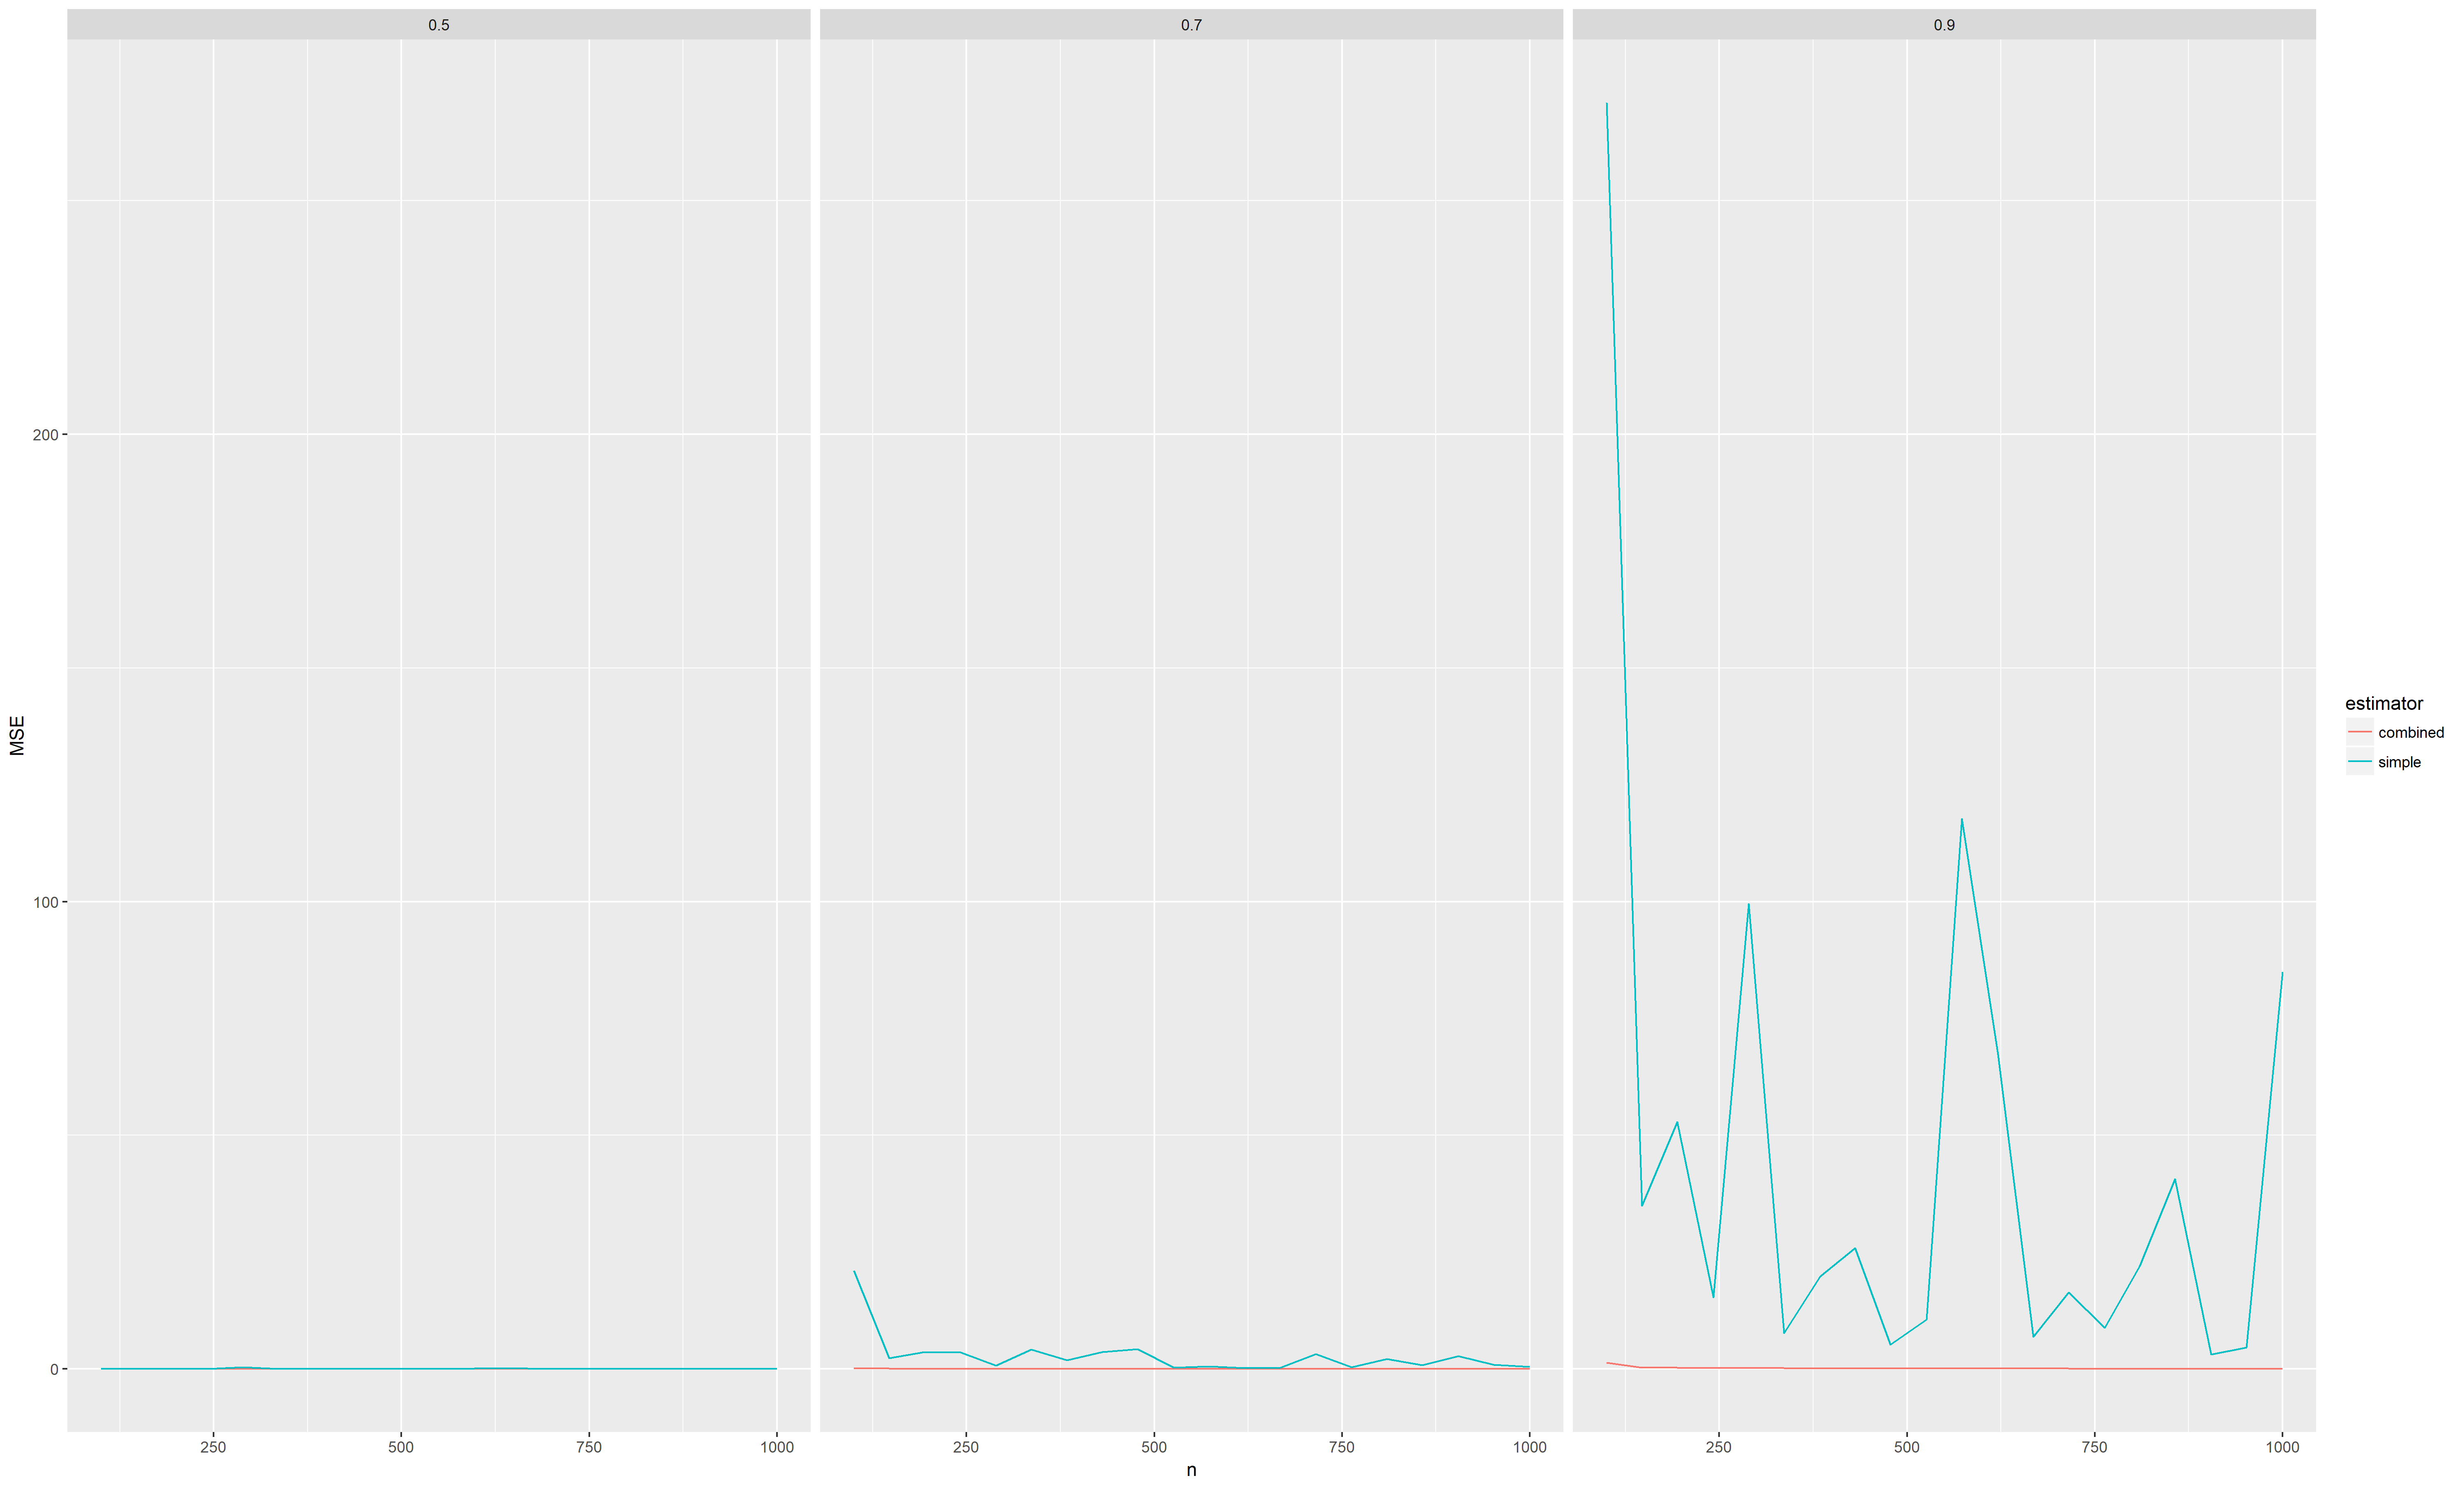
\includegraphics[width=\linewidth]{041118a.png}
  \caption{MSEs of two approaches compared. The simple estimator looks
  almost inconsistent for $p=.9$ but see fig. \ref{fig:2}.}  \label{fig:1}
\end{figure}
\begin{figure}[h!]
  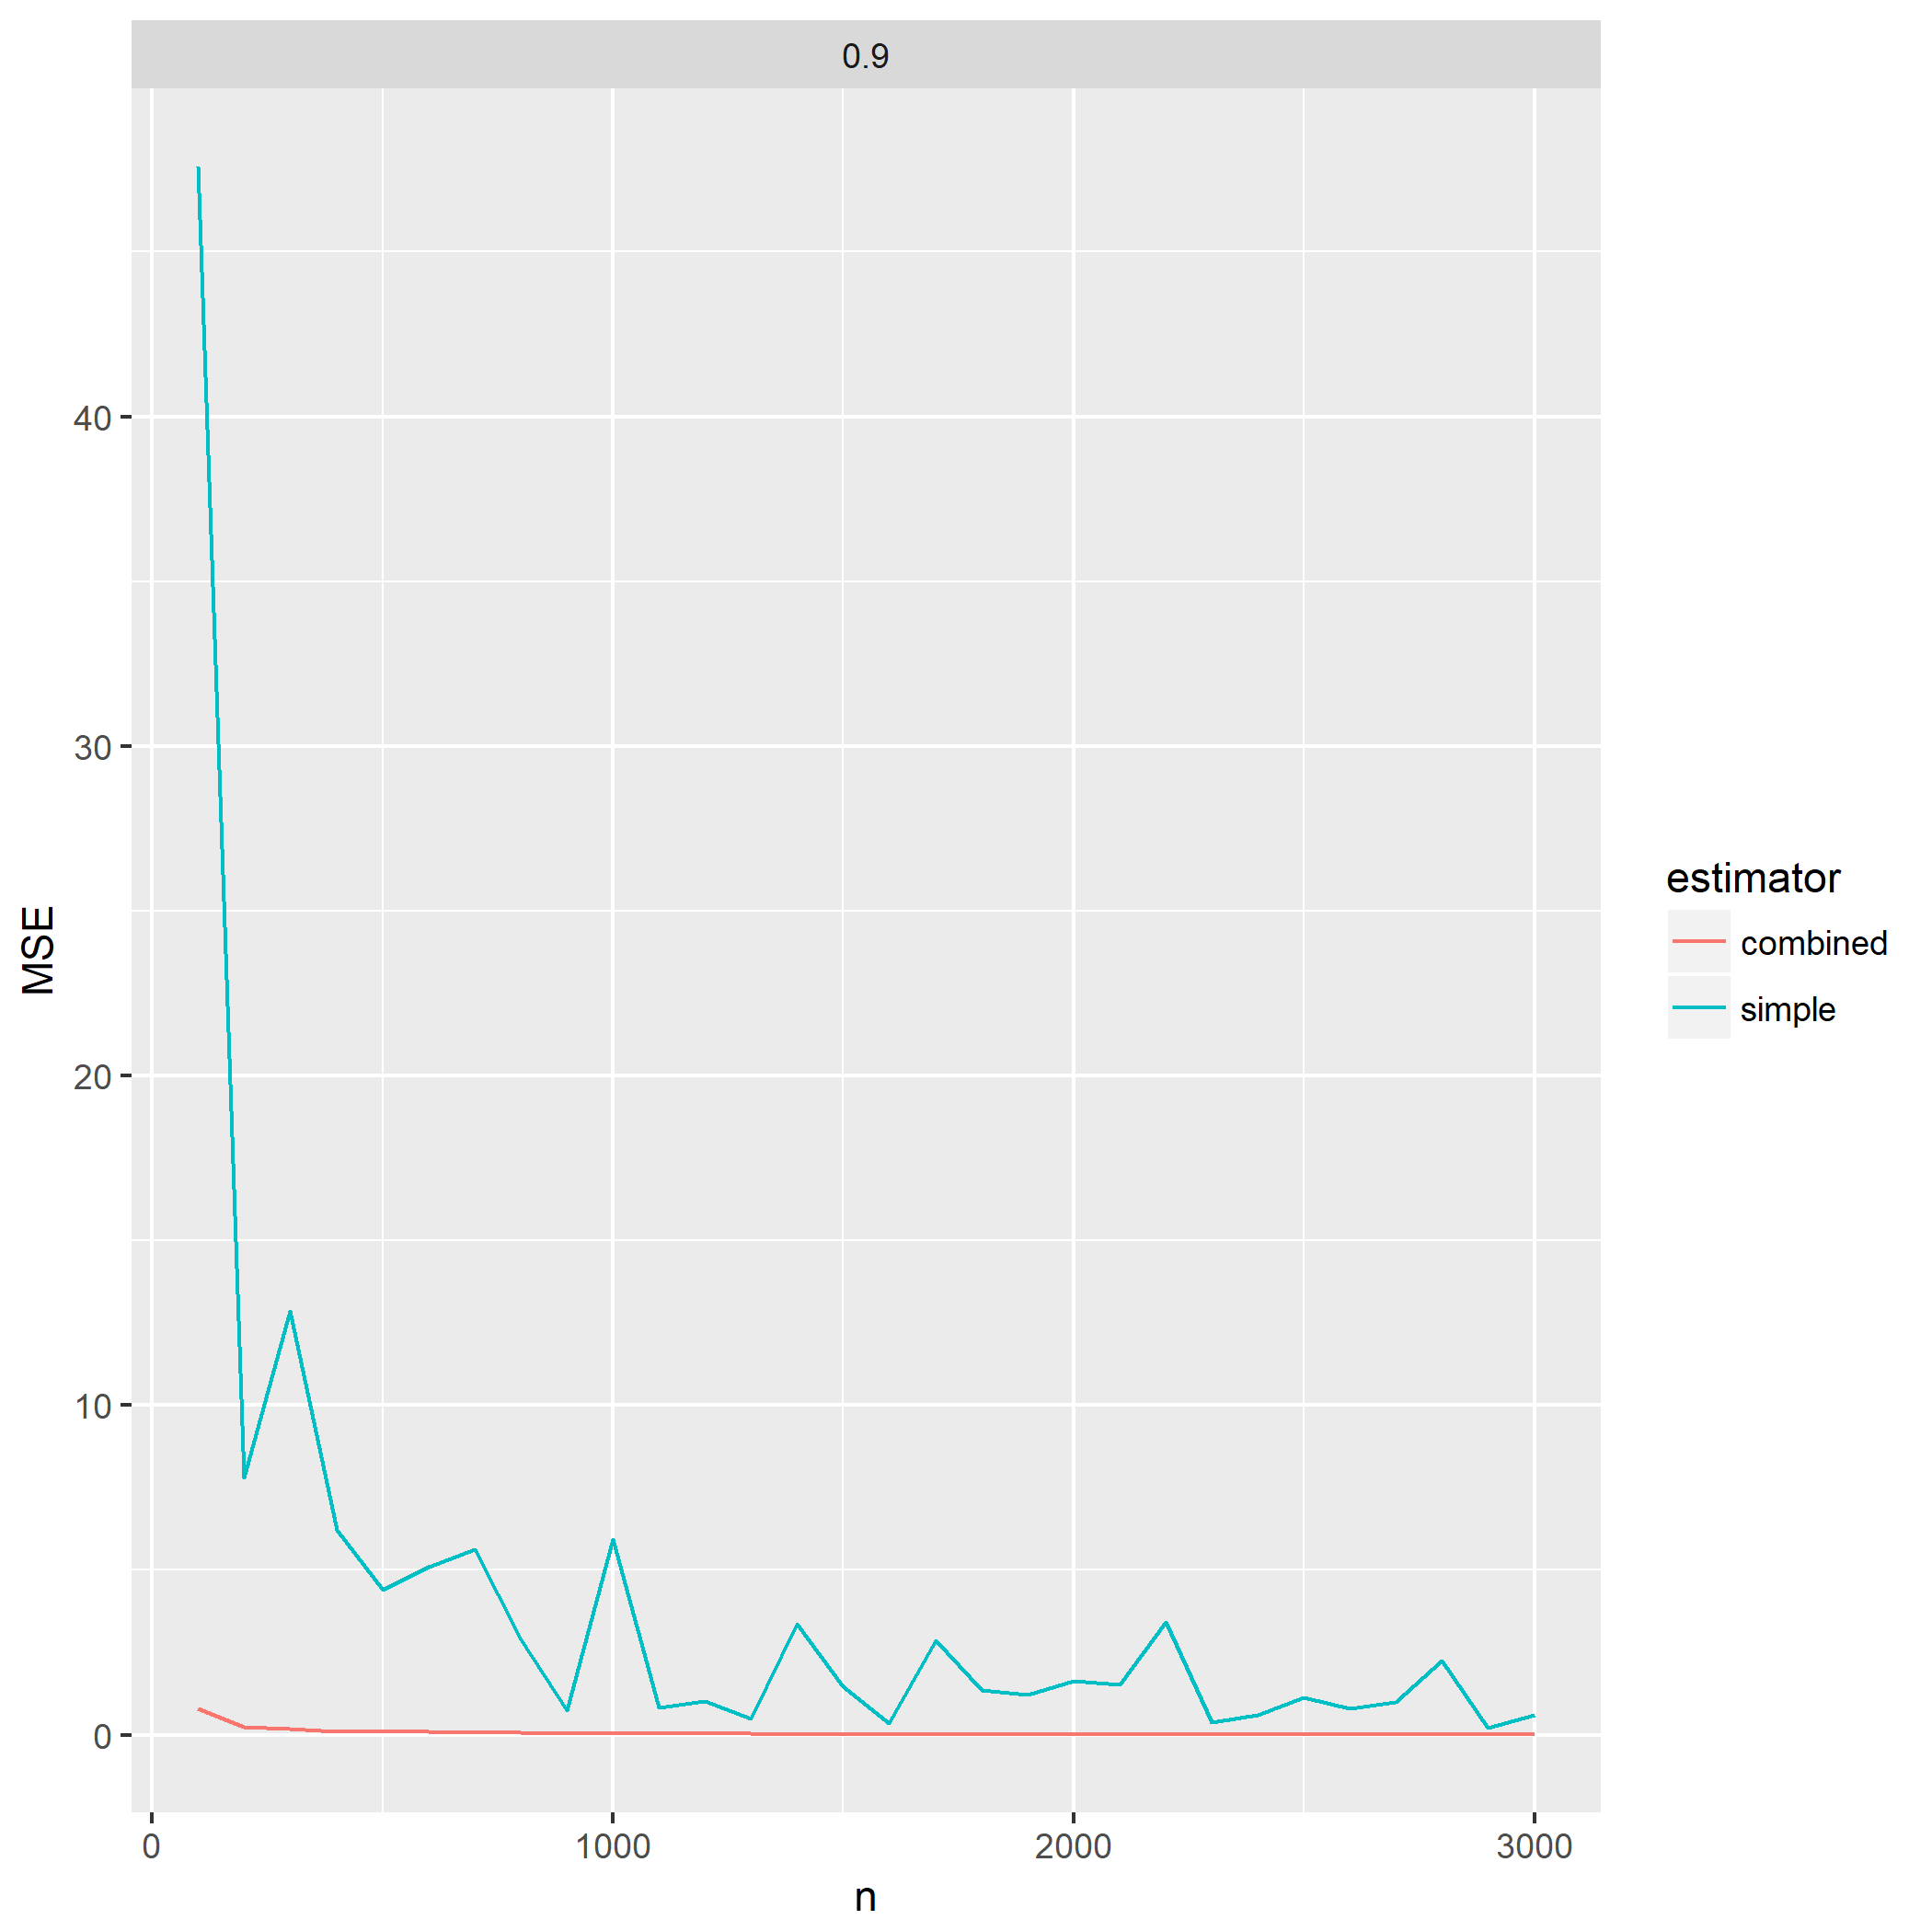
\includegraphics[width=\linewidth]{041118b.png}
  \caption{Focusing on the problematic case of $p$ close to 1
    (symmetric for $p$ close to 0.}  \label{fig:2}
\end{figure}

The OLS estimators are used in both approaches here. The case and
control data satisfy the OLS assumptions, e.g., the case data
follows
\[
  Y = \alpha + \beta^TX + \epsilon.
\]
For the proposed approach, the data follows
\begin{align}
  \tilde{Y} = \left(\frac{p}{1-p}\right)^{1-2A}Y = \left(\frac{p}{1-p}\right)^{1-2A}\alpha A +
  \left(\frac{p}{1-p}\right)^{1-2A} \beta^TX + \left(\frac{p}{1-p}\right)^{1-2A}\epsilon,
\label{eqn:re}
\end{align}
which looks like a random intercept, random slope model with two levels. But
because of the orthogonality of $A$ and $X$, still
\[
  \EE(\tilde{Y}\mid X) = \alpha' + \beta^T X
\]
so the OLS estimator should be efficient for the transformed
data.

Does this seem right to you, that this inefficiency is
unavoidable for the simple linear model? By the way, the difference between the
two approaches seems to go away with interaction terms. In that case
the Tsiatis approach also has a random effects form that we are
marginalizing over, similar to $(\ref{eqn:re})$.


\end{document}


